\documentclass[reprint, amsmath,amssymb, aps,pra]{revtex4-1}

\usepackage[utf8]{inputenc}
\usepackage[draft,inline,nomargin]{fixme}
\usepackage{graphicx}
\usepackage{dcolumn}
\usepackage{bm}
\usepackage{braket}



\begin{document}

%\preprint{APS/123-QED}

\title{Optomechanical cooling with time-dependent parameters}%

\author{Pablo Yanes-Thomas}

\author{Marc Bienert}

\author{Pablo Barberis-Blostein}

\affiliation{Instituto de Investigaciones en Matem\'{a}ticas Aplicadas y en Sistemas,
Universidad Nacional Aut\'{o}noma de M\'{e}xico, Circuito Escolar s/n Ciudad Universitaria M\'{e}xico, D.F.}%



\date{\today}

\begin{abstract}
  We model the laser cooling of a parametrically driven optomechanical
  cavity using a dissipation model 
  that accounts for the modification of the quasi-energy spectrum
  caused by the driving. We construct a master equation for the
  mechanical object using Floquet operators. When the natural
  frequency of the mechanical object oscillates periodically around its mean value,
  we derive, using an adiabatic approximation, an analytical
  expression for its temperature. This expression depends both on the
  oscillator's mean frequency and that of the frequency's oscillations
  around its mean value. We find that the temperature can be lower
  than in the non-time dependent case. Our results raise the
  possibility of achieving lower temperatures for the mechanical object
  if its natural frequency can be controlled as a function of time.
\end{abstract}

\pacs{Valid PACS appear here}% PACS, the Physics and Astronomy
                             % Classification Scheme.
%\keywords{Suggested keywords}%Use showkeys class option if keyword
                              %display desired
\maketitle

%\tableofcontents

\section{Introduction}


Quantum cavity optomechanics studies systems composed of macroscopic
mechanical objects, such as mirrors, and an optical cavity's quantized light field
usually coupled via radiation pressure.
In a common scheme an end-mirror of a Fabry-Perot
cavity is suspended while being able to freely oscillate.
When photons are reflected by the mirror, there is a
momentum transfer between the light field and the mirror and hence a coupling force. As the cavity's
resonance depends on its length, the mechanical
displacement affects the light field inside the cavity. Some of the first theoretical work predicting this sort of coupling was performed by \cite{BraginskiiOG}. This interaction between
the macroscopic mechanical object and the light field leads to several
interesting effects such as optomechanically induced
transparency \cite{WeissOIT}, the optical spring effect \cite{VogelOT}
or, most relevant to this study, optomechanical
cooling \cite{CohadonCM, CorbittOC, SchliesserRPC, LCNooshi}.
	
Optomechanical cooling was first proposed by Mancini, et al in
\cite{ManciniOC}. It is the damping of the end mirror's mechanical
motion due to the radiative coupling to the cavity field. Sideband cooling takes place when the cavity's resonance is much narrower than the mechanical frequency. It can be understood as Raman scattering
\cite{MarquardtQTOQ} of incident photons, red-detuned from the
cavity resonance, when the parameters are chosen to favor phonon absorption from the mechanical oscillator in order to scatter the photon
into the cavity's resonance mode, resulting in cooling. For coherent quantum control over a mechanical object, it must be
close to a pure quantum mechanical state \cite{KippenberCO} so
effective methods of cooling macroscopic objects to low temperatures is highly desirable.

One possible avenue for improved cooling lies in controlling the
mechanical resonator's frequency as a function of time
\cite{JockelMR}. The effect of this dependence on the mechanical
object's final temperature was studied in \cite{BarberisLC}. In that
study it was found that the final temperature of the parametrically
driven harmonic oscillator was larger than the nondriven case.
The master equation from which the cooling rates were derived,
accounted for the natural frequency of the mechanical
resonator via ad-hoc time-dependent coefficients. These were
introduced after performing the Markov approximation. This approach
could lead to an incomplete master equation and thus an incomplete
description of the system's dynamics, as the system is being treated
as essentially not time-dependent during the derivation of the master
equation. In this study, we employ a different method that accounts
for the time dependence throughout the entire derivation.


The formalism which we apply (section \ref{OptmechH}) is based on
Floquet theory and was demonstrated to be a more accurate treatment in
\cite{HanngiFM}. For the case where the drive consist of a small
periodic oscillation with respect to the central frequency of the
mechanical oscillator, the Floquet operators can be given explicitly
(section \ref{SolSmallOsc}). Under the adiabatic approximation, we
derive an approximated expression for the
mean phonon occupation number in the final stages of optomechanical cooling (section \ref{LasCool}). We perform numerical
calculations in order to compare this expression to the one for the
non-time-dependent case (section \ref{NumCal}). We find, using the
formalism  presented here, that lower temperatures can be obtained if
the mechanical object is parametrically driven. Our results suggest
that the theoretical model of dissipation of the mechanical osscilator
can have a significant influence on the resulting temperature. (section \ref{ConCl}).


% The formalism which we apply is based on Floquet theory and was
% demonstrated to be a more accurate treatment in \cite{HanngiFM}. We
% obtain a master equation expressed in terms of Floquet operators and
% from there derive an approximated expression for the final mechanical
% state's mean phonon occupation number, which is used as a proxy for
% the state's temperature, under the adiabatic approximation. We perform
% numerical calculations in order to compare this expression to the one
% for the non-time-dependent case.

%We study the cooling of a macroscopic mechanical harmonic oscillator
%with time-dependent natural frequency coupled to an optical cavity's
%light field via radiation pressure when the mechanical oscillator's
%natural frequency varies periodically in time with a small amplitude
%vis-a-vis a constant central frequency. Typically \cite{BarberisLC},
%the interaction between the two systems is too small for the cooling
%to be faster than the system's re-thermalization, so a laser, which
%acts as a photon pump, is employed to boost the interaction.

% The paper is structured as follows. In section \ref{OptmechH}, a
% Hamiltonian for optomechanical cooling for the time-dependent harmonic
% oscillator is presented and expressed in terms of time-dependent
% operators and in a displaced reference frame. In section
% \ref{SolSmallOsc}, we calculate explicit expressions  for the specific case of small periodic oscillations. The
% corresponding master equation is obtained in terms of these explicit
% expressions under the Markov approximation. In section
% \ref{LasCool}, we derive a master equation under the adiabatic
% approximation for only the mechanical degrees of freedom and obtain an
% explicit expression of the mean vibrational occupation number as a
% measure of the final state's temperature. Finally, we compare the
% temperature prediction for the non-time dependent case to the new
% prediction obtained in this study.

\section{Optomechanical Hamiltonian}\label{OptmechH}
\subsection{Hamiltonian with Floquet Operators}
	
	We employed the standard Hamiltonian for optomechanical cooling \cite{LCNooshi} in a reference system that rotates with the same frequency as a laser that continuously pumps photons into the cavity. 

\begin{equation}
H(t) =   H_{cav} + H_{mec}(t) + H_{int} + H_{pump},
\end{equation}

where

\begin{align}
H_{cav} =& -\hbar \delta a^\dagger a,\\
H_{mec}(t) =& \frac{p^2}{2M} + \frac{1}{2}M \nu^2 (t) x^2,\\
H_{int} =& -\hbar g a^\dagger a x,\\
H_{pump} =& \hbar\frac{\Omega}{2}(a^\dagger + a),
\end{align}
$\delta = \omega_{laser} - \omega_{cav}$ is the frequency difference
between the laser and the cavity. $M$ is the mechanical oscillator's
mass and $\nu(t)$ is its frequency. In order to employ the Floquet
formalism $\nu(t)$ must be a periodic function of time. The $H_{int}$
term models the interaction between photons and the mirror, and $g$
sets the strength of the coupling. Finally, $\Omega$ describes the strength
of the cavity pump. Readers interested in a derivation of the
interaction term should consult \cite{KippenberCO}. In our case, the only term with
an explicit time dependence is the term for the mechanical oscillator.

The Floquet operators are analogous to the usual creation and annihilation operators for the standard harmonic oscillator and can be expressed in terms of the
mechanical oscillator's position and momentum operators \cite{HanngiFM}. These operators are

\begin{equation}\label{FloquetOperators}
\Gamma(t) = \frac{1}{2i}\left[\hat{x}\sqrt{\frac{2M}{\hbar}}\dot{f}(t)-\hat{p}\sqrt{\frac{2}{M \hbar }}f(t)\right],
\end{equation} as well as its Hermitian conjugate. $f(t)$ is the solution to the classical time-dependent harmonic oscillator equation of motion in one dimension and is generally a complex function \cite{BrownPT}

\begin{equation} \label{TimeDependentHO}
\ddot{f} + \nu(t)^2f=0.
\end{equation} This equation has two solutions \cite{HanngiFM} of the form
\begin{equation}
f(t) = e^{i\mu t}\phi(t), 
\end{equation} and its complex conjugate. $\phi(t)$ is a periodic function of time with the same period as $\nu(t)$.  $\mu$ is, in general, a complex number \cite{WardFT}. These operators follow the usual commutation relations for creation and annihilation operators
\begin{equation}
[\Gamma(t)^\dagger,\Gamma(t)]=1.
\end{equation}

 Using these operators $H_{mec}(t)$ can be written in the same form as the non time-dependent harmonic oscillator with the Floquet operators taking the place of the annihilation operators, with the exception of a global time-dependent scalar coefficient  \cite{BrownPT}

\begin{equation}
H_{mec}(t) = \hbar\frac{W}{|f(t)|^2}\left[\Gamma^\dagger(t)\Gamma(t) + \frac{1}{2}\right],
\end{equation}
with the Wronskian $W$ for \eqref{TimeDependentHO}. Equation
\eqref{FloquetOperators} is then inverted and solved for the harmonic
oscillator's position operator \cite{TesisMaestria}

\begin{equation}
\hat{x} = \frac{b^* \Gamma - b\Gamma^\dagger}{(b^*a-ba^*)}
\end{equation} with

\begin{align}
a =&  \frac{1}{2i}\sqrt{\frac{2M}{\hbar}}\dot{f}\, , \\
b =&  \frac{1}{2i}\sqrt{\frac{2}{M\hbar}}f\, .
\end{align}
These are then substituted back into the interaction Hamiltonian
resulting in

\begin{equation}
H_{int}(t) = g\sqrt{\frac{\hbar}{2M}}a^\dagger a[\gamma_+(t)\Gamma (t) +\gamma_-(t)\Gamma^\dagger (t)],
\end{equation} with new coefficients

\begin{align*}
\gamma_+(t)=&\frac{f^*}{(f^*\dot{f}-f\dot{f}^*)},\\
\gamma_-(t)=&\frac{f}{(f^*\dot{f}-f\dot{f}^*)}\, .
\end{align*} 


The Hamiltonian contains two separate harmonic oscillator-like terms
that commute with each other, $H_{cav}$ and $H_{mec}$, so the standard
harmonic oscillator master equation structure can be employed
\cite{TesisMaestria}\cite{HanngiFM}. The usual derivation of the master
equation involves a Markov approximation, under the formalism we
employ, frequency's time dependence is accounted for during this
approximation \cite{HanngiFM} via the Floquet operators. This differs
from previous attempts to study this type of system, where this
dependence was included after the Markov approximation had been
performed via time-dependent ad-hoc coefficients for the damping
\cite{BarberisLC}. As demonstrated in \cite{HanngiFM}, the method
employed here is a more complete, and thus accurate, treatment.

The corresponding master equation is
\begin{equation} \label{LCMasterEquation}
\dot{\rho} = \frac{1}{i\hbar}[H,\rho] +L_a\rho + L_\Gamma \rho,
\end{equation}
where
\begin{align}
L_a \rho =& - \frac{\kappa}{2}(n_p + 1)[a^\dagger a\rho + \rho a^\dagger a -2a\rho a^\dagger]  \\
 &- \frac{\kappa}{2}(n_p)[ aa^\dagger\rho + \rho  aa^\dagger -2a^\dagger\rho a]\, ,\nonumber
\end{align}

\begin{align}\label{eq:mechanical_dissipation}
  L_\Gamma \rho =& - \frac{\gamma}{2}(n_m + 1)[\Gamma^\dagger \Gamma\rho + \rho \Gamma^\dagger \Gamma -2\Gamma\rho \Gamma^\dagger]  \\
                 &- \frac{\gamma}{2}(n_m)[ \Gamma\Gamma^\dagger\rho + \rho  \Gamma\Gamma^\dagger -2\Gamma^\dagger\rho \Gamma]\, ,\nonumber
\end{align} 
$\kappa$ is the energy decay rate for the cavity and $\gamma$ is the
decay rate for the mechanical oscillator. The number of thermal
excitations for the cavity and the oscillator are given by $n_p$ and
$n_m$ respectively \cite{EnglertFL}. The superoperators $L_\Gamma$ and
$L_a$ model the energy exchanges between the environment and the
cavity and the mechanical resonator respectively. The formalism
developed in \cite{HanngiFM} was used to derive the mechanical
dissipation term \eqref{eq:mechanical_dissipation}.

Equation \eqref{LCMasterEquation} represents a master equation for a
parametric optomechanical system with an improved dissipation model
which accounts for the mechanical oscillator's time dependent
frequency.



\subsection{Displaced Frame}

In order to eliminate the pump term and to find useful
  approximations, we employ a unitary transformation to
shift \eqref{LCMasterEquation} into a displaced reference frame. This
transformation depends on two time-dependent coefficients, $\alpha(t)$
and $\beta(t)$, which are chosen in a convenient manner to simplify
the Hamiltonian. The transformation is given by the operator
\begin{equation}\label{ShiftTransform}
U_{a,\Gamma} = e^{(\alpha(t) a^\dagger - \alpha^*(t)a)}e^{(\beta(t) \Gamma^\dagger - \beta^*(t)\Gamma)},
\end{equation}
and results in a displaced Hamiltonian and in turn a displaced master
equation
\begin{equation}
\dot{\rho}' = \frac{1}{i\hbar}[H',\rho'] +L_a\rho' + L_\Gamma \rho' + C(t)\rho'\, ,
\end{equation}
for the time evolution of the density operator $\rho'(t)$ which
represents the coupled cavity-mechanical resonator system. The primes
indicate that the transformation has been applied. The displaced
Hamiltonian, which includes a pump-like term that appears when making the
transformation on the $L$ operators, is given by
\begin{align*}
  H'=& -\hbar \delta' a^\dagger a + \hbar\frac{W}{|f(t)|^2}\Gamma \Gamma^\dagger\\
     &-\hbar g\sqrt{\frac{\hbar}{2M}}[(a^{\dagger}a +\alpha a^{\dagger}+\alpha^* a)(\gamma_-(t)\Gamma^{\dagger}+\gamma_+(t)\Gamma)]\\
     &+ i\hbar(\beta^*\dot{\Gamma} - \beta \dot{\Gamma}^\dagger),
\end{align*}
with $\delta' = \delta + g\sqrt{\frac{\hbar}{2M}}(\beta + \beta^*)$.
This Hamiltonian is valid as long as the coefficients $\alpha(t)$ and
$\beta(t)$ fulfill the differential equations

\begin{align}
\dot{\alpha} =& \alpha(-\frac{\kappa}{2}+i(\delta+g\sqrt{\frac{\hbar}{2M}}(\gamma_-(t) \beta^* + \gamma_+(t) \beta))-i\frac{\Omega}{2},\\
\dot{\beta} =& \beta(-\frac{\gamma}{2}-i\frac{W}{|f(t)|^2})+ig\sqrt{\frac{\hbar}{2M}}|\alpha|^2\gamma_+(t).
\end{align}


The $C(t)$ term
 \begin{align}
C(t)\rho = |\beta|^2(C(t)_{+-} - C(t)_{-+})\rho \nonumber,
 \end{align}
 where
\begin{align*}
C(t)_{+-} =& [\dot{\Gamma}^{\dagger}, \Gamma],\\
C(t)_{-+} =& [\dot{\Gamma}, \Gamma^{\dagger}],
\end{align*}
appears because the Floquet operators do not necessarily commute with
their own time derivatives. In the case of the Hamiltonian for the
cavity's light field, the operators contain no explicit time
dependence. The Floquet operators, however,
do include such a dependence, which introduces additional terms into
the master equation. These terms involve the commutators between the
Floquet operators and their time derivatives and contain no operator
dependence whatsoever and as such are not considered part of the
Hamiltonian. These commutation relations are not, in general, zero
\cite{TesisMaestria}, they depend on the specific form of the
solutions for \eqref{TimeDependentHO}, $f$ and $f^*$. For example

\begin{equation}
C(t)_{-+} = -(C(t)_{+-})^* = \frac{i}{2}(\dot{f}^* \dot{f} - \ddot{f}^*f^*).
\end{equation}



Proceeding further requires an explicit solution for
\eqref{TimeDependentHO}. The primes in the operators will be omitted
from now on as all calculations will be done in the displaced frame.


\section{Solution for Small Oscillations}\label{SolSmallOsc}
 
In order to obtain an explicit form of the Floquet operators, we focus
on the case of small oscillations around a central frequency,
specifically\fxnote{Pablo: cambie notacion, checalo.}

\begin{equation}\label{SmallOscillationsTDHO}
\nu(t) = \nu_0 + \epsilon' cos(2\omega t),
\end{equation}
with $\epsilon' \ll \nu_0$ where $\nu_0$ is the mean frequency.


With these expressions we may solve for the $\alpha(t)$ and $\beta(t)$ coefficients. The equations are

\begin{align}
\dot{\alpha} =& \alpha(-\frac{\kappa}{2}+i(\delta+g\sqrt{\frac{\hbar}{2M}}(e^{i\omega t} \beta^* + e^{-i\omega t} \beta))-i\frac{\Omega}{2},\\
\dot{\beta} =& \beta(-\frac{\gamma}{2}-i 2\omega)+ig\sqrt{\frac{\hbar}{2M}}|\alpha|^2e^{i\omega t},
\end{align}
however our focus is on the stationary case
($\dot{\alpha}(t)=\dot{\beta}(t)=0$) and in a weak coupling regime, so
coefficients of first order in $g$ or higher are neglected, which
results in two simplified equations

\begin{align}
0 =& \alpha(-\frac{\kappa}{2}+i\delta)-i\frac{\Omega}{2},\\
0 =& \beta(-\frac{\gamma}{2}-i 2\omega),
\end{align} which are trivially solved 

\begin{align}
\alpha_0 =& \frac{\Omega}{2\delta-i\kappa},\\
\beta_0 =& 0.
\end{align} The 0 sub-index denotes that the solutions are valid only to zeroth order in the coupling parameter. 

\subsection{Laser Cooling Hamiltonian}

Under these parameters we can neglect the $C(t)$ terms as they
figure into the
master equation as terms of first order in $\epsilon$ and second order
in $\beta$. The term involving the time derivatives of the Floquet
operators can also be neglected for this reason. The Hamiltonian can
then be written as

\begin{align}
H =& -\hbar \delta a^{\dagger}a +\hbar\omega\Gamma^{\dagger}\Gamma \\
&-\hbar g\sqrt{\frac{\hbar}{2M}}(a^{\dagger}a +\alpha_0 a^{\dagger}+\alpha^*_0 a)(\gamma_-(t)\Gamma^{\dagger}+\gamma_+(t)\Gamma)\nonumber.
\end{align} We focus on the case where $|\alpha_0| \gg 1$
\cite{BarberisLC}, so that the $a^\dagger a$ term can be neglected as
it is small when compared to the other two terms in the interaction.
This leads to a further simplified Hamiltonian

\begin{align} \label{LCHamiltonian}
H(t) =& -\hbar \delta a^{\dagger}a +\hbar\omega\Gamma^{\dagger}\Gamma \\
&+\frac{\hbar g\sqrt{\frac{\hbar}{2M}}}{\omega}(\alpha_0 a^{\dagger}+\alpha^*_0 a)(e^{i\omega t} \nonumber\Gamma^{\dagger}+e^{-i\omega t}\Gamma).
\end{align}
This Hamiltonian corresponds to a standard optomechanical master
equation with Floquet operators for the mechanical oscillator


\begin{equation}\label{LCMasterEq}
\dot{\rho} = \frac{1}{i\hbar}[H,\rho] +L_a\rho + L_\Gamma \rho,
\end{equation} where $L_a$ corresponds to the cavity's light field \cite{ZollerQN} and $L_\Gamma$ corresponds to the time dependent harmonic oscillator \cite{HanngiFM}.


\section{Laser Cooling}\label{LasCool}

Our focus is on the parameter regime where the mechanical resonator's
temperature evolves much more slowly than the cavity's losses and than
the mechanical frequency. This requires
$(g\sqrt{\frac{\hbar}{2M}}\alpha_o)^2 \ll (\frac{\kappa}{\omega_m})$. Following the
derivation found in \cite{LCNooshi}, we arrive at a master equation
for the density operator, after projecting into the subspace corresponding to
its stationary state and tracing over the cavity degrees of freedom. The technical details of the derivation is reported in App.~\ref{CoolingAppendix}. It leads to the master equation 
\begin{equation}\label{eq:projected_master_equation}
\dot{\mu}\approx -\frac{g'^2}{2}G(\nu_m,n_c)[\Gamma^\dagger,\Gamma\mu]-G^*(-\nu_m,n_c)[\Gamma^\dagger,\mu\Gamma],
\end{equation} where we have set $g'=g\sqrt{\frac{\hbar}{2M}}\alpha_0$  for convenience and use $\mu$ as the density operator of the mechanical degree of freedom. The
cavity-quadratures correlation $G(\nu_m,n_p)$ can be used to calculate the heating and cooling rates
for the mirror and is given by
\begin{equation} \label{CavityQuadrature}
G(\nu_m,n_p) = \int_0^\infty dt e^{i\nu(t) t}Tr_a[X_a e^{L_a t} X_a \rho_{st}],
\end{equation} with 
\begin{equation}
X_a = \frac{a + a^\dagger}{\sqrt{2}\alpha_0},
\end{equation}

the cooling and heating rates are given by


\begin{equation}
A_\pm(\nu_m,n_p) = g'^2Real(G(\mp \nu_m,n_p)),
\end{equation} where $A_+$ represents heating and $A_-$ represents cooling. The final number of phonon excitations is given by

\begin{equation}
\langle m \rangle =\langle \Gamma^\dagger \Gamma \rangle = \frac{A_+}{A_- - A_+}.
\end{equation}

Thus if \eqref{CavityQuadrature} can be calculated, the heating and
cooling rates and the final temperature (represented by the
average number of phonon excitations) can be obtained in a
straightforward manner. This procedure is done numerically in the
following section.

\fxnote{Una de las cosas mas bonitas es que desaparece la referencia a
  la solucion de las ecuaciones de Mathieu en la aproximacion
  adiabatica. Pon un parrafo explicando donde, porque  y cuando pasa esto.}
\section{Calculation of Mean Vibrational Occupation Number}\label{NumCal}

To perform numerical computations we calculate
\eqref{CavityQuadrature} up to first order in $\epsilon$. We assume
that the cavity is at zero temperature ($n_p=0$).  The trace inside
\eqref{CavityQuadrature} can be easily calculated, we obtain
\begin{align}
G(\nu,0)=&\int_0^\infty dt e^{(i\nu(t)) t}Tr[...]\nonumber\\
&= \int_0^\infty e^{i(\nu_0 + \epsilon cos(2\omega t) )t} Tr[...]dt, \nonumber\\
&=\int_0^\infty e^{i \nu_0 t}e^{i \epsilon cos(2\omega t)t} Tr[...]dt, \nonumber\\
&\approx \int_0^\infty e^{i \nu_0 t}(1+i \epsilon cos(2\omega t)t) Tr[...]dt, \nonumber\\
&=\int_0^\infty e^{i \nu_0 t}Tr[...]dt\nonumber\\
&+i\epsilon\int_0^\infty cos(2\omega t)t e^{i \nu_0 t}Tr[...]dt\, ,\nonumber
\end{align}The $Tr[...]$ can be evaluated in a straightforward manner and results in

\begin{equation}
Tr_a[X_a e^{L_a t} X_a \rho_{st}] = \frac{1}{2}e^{-(\frac{\kappa}{2}-i\delta) t},
\end{equation} the $e^{-\kappa t}$ factor acts as a cut-off for the integral, which allows for the expansion to be performed. See Appendix \ref{App1} for more on the eigenvalues of the trace states.
This leads to an expression for \eqref{CavityQuadrature} which consist
of two parts: one corresponding to the nondriven harmonic oscillator
case plus a correction term proportional to $\epsilon$
\begin{equation}
\frac{G(\nu,0)}{g'^2}= \frac{1}{-\kappa + 2i(\delta + \nu_0)} +i\epsilon\frac{(-\kappa + i(\nu_0 + \delta))^2 - 4\omega^2}{((-\kappa + i(\nu_0 + \delta))^2 + 4\omega^2)^2}\, .
\end{equation} %where  $E_0 = g \sqrt{\frac{\hbar}{2m\nu_0}}$.

We evaluate the real part of this expression numerically. In order for
the adiabatic approximation to be valid, the variation in the
mechanical oscillator's frequency must be slow when compared to the
frequency itself ($\omega \ll \nu_0$) which translates to classical
solutions with $1 \ll n$ due to \eqref{scattering}. Assuming that
$\epsilon = \frac{\nu_0}{10}$ we now have the condition
$\epsilon = \frac{n^2}{5}$. We wish for $n$ to be sufficiently large
so as to fulfill the condition relating $\nu_0$ and $\omega$ but small
enough so that $\epsilon \ll \nu_0$. To this end we chose
$n=\sqrt{\frac{\nu_0}{2}}$ (rounded to the nearest integer) which
maintains the previous ratio between the two frequencies. Physically,
we employ a classical solution which describes a situation where the
oscillator's average $\nu_0$ frequency is the fastest one, while the
secular frequency $\omega$ is of the order of the perturbation
frequency $\epsilon$. In figure \ref{GraficaTemp} it is shown the
number of mechanical oscillations when $\frac{\delta}{\nu_0}$ is in
the range of $[-2,2]$. Compared with the non-driven case, the
parametrically driven oscillator has a frequency shift of where to
expect the minimum number of excitations, and a region where the
predicted number of excitations is smaller. The reason of this
behavior is that, as $\epsilon$ increases, the parametric modulation
causes the cooling and heating coefficients to shift away from each
other, and its distribution becomes narrower and presents a higher
peak. This can be observed in figure \ref{GraficaA-}. As long as
$\nu_0$ and $\omega$ fulfill \eqref{scattering}, altering them does
not change the final temperature. The parameters used are consistent
with the reported controlled frequency modulation
\cite{WoolleyNM}\cite{JockelS}. \fxnote{Pablo: Doble checa que esto
  sea verdad}



\begin{figure}
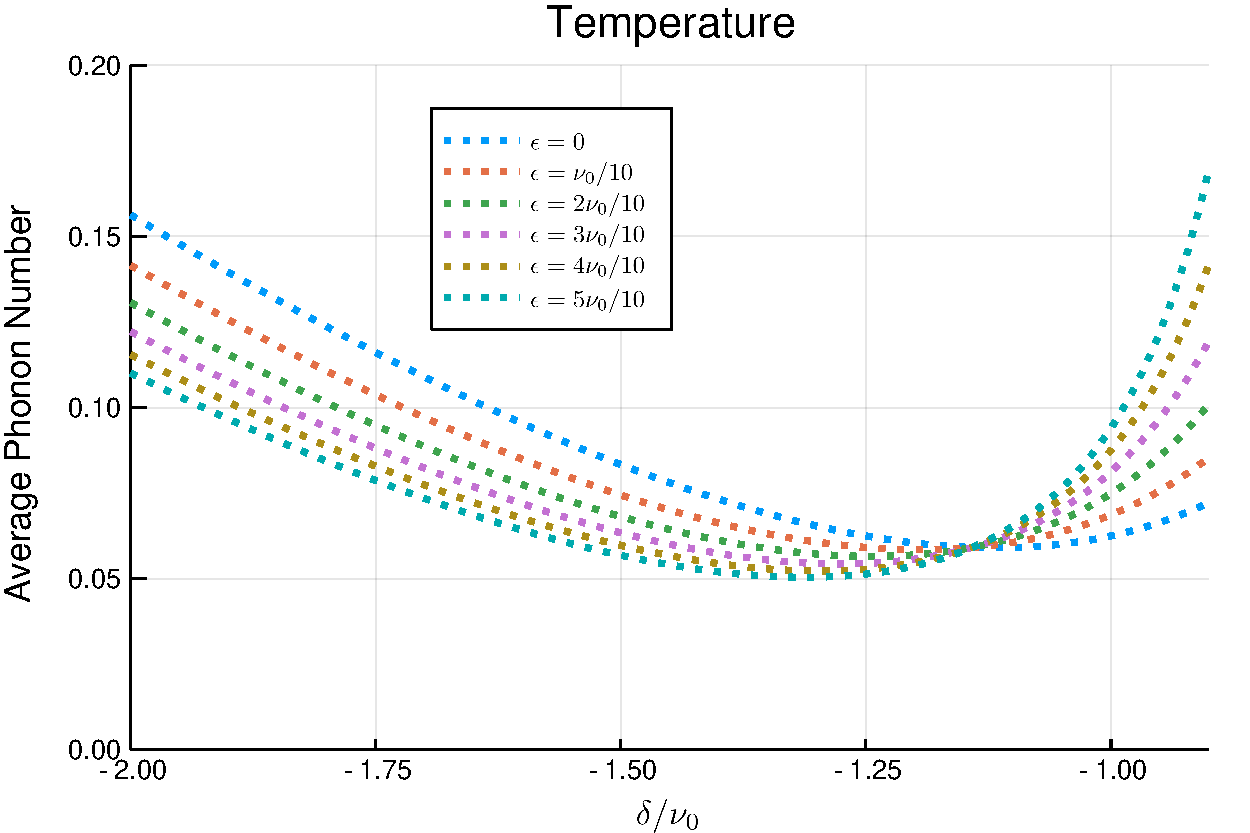
\includegraphics[scale=.4]{Temperature.pdf}  
\caption{ Mechanical oscillator phonon number as a function of the
  perturbation. The correction results in a shift of the location of
  the minimum temperature, as well as a lower minimum. All curves
  cross the same point. We used the parameters in the text plus
  $\kappa \ll \nu_0$}
\label{GraficaTemp}
\end{figure}

\begin{figure}
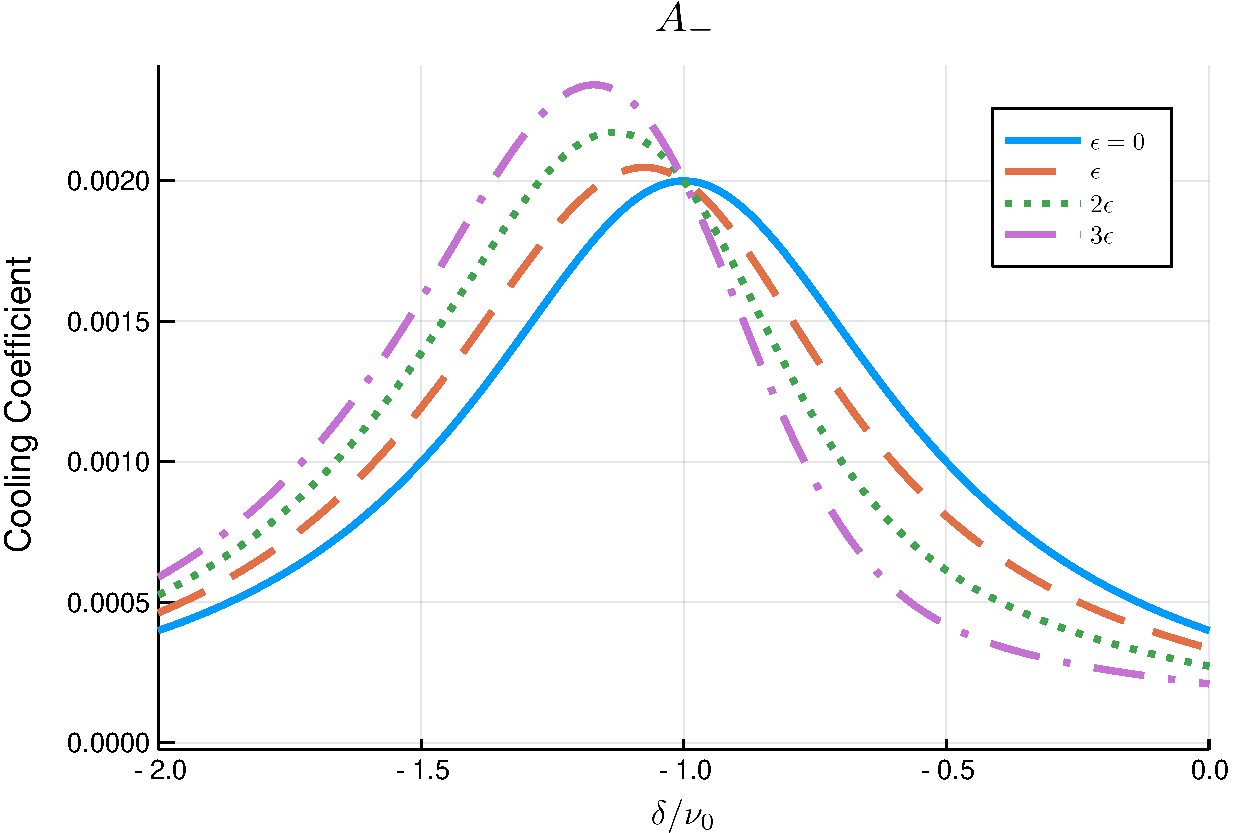
\includegraphics[scale=.4]{GraficaA-.pdf}
\caption{Cooling coefficient $A_-$ as a function of the perturbation.
  As $\epsilon$ increases the $A_-$ presents a narrower distribution
  and a higher peak. The peak shifts away from the cavity resonance
  corresponding to $\nu_0$. $A_+$ is not shown as, in this region, it
  is around 4 orders of magnitude smaller than $A_-$. We used the
  parameters in the text plus $\kappa \ll \nu_0$.}
\label{GraficaA-}
\end{figure}



% \begin{figure}
% 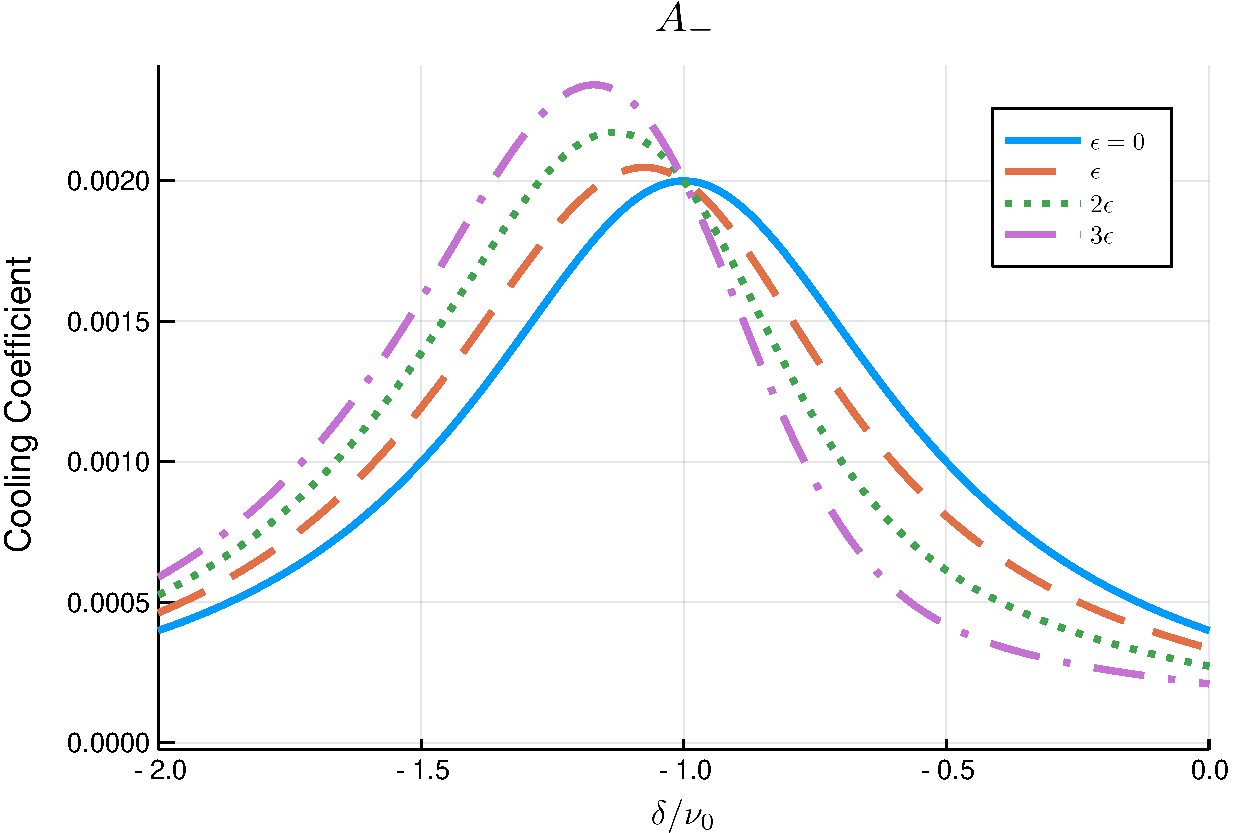
\includegraphics[scale=.4]{GraficaA-.pdf}
% \caption{Cooling sideband for different perturbation levels. Besides all the scattering relations already stated, we
%   work under $\kappa \ll \nu_0$}
% \label{GraficaA-}
% \end{figure}





\section{Conclusions}\label{ConCl}

Using an improved theoretical description of dissipation of a
parametrically driven mechanical object, in an optomechanical setup,
we found that the lowest temperature reached can be lower than in the
non-driven case. This implies that periodically changing the natural
frequency of the mechanical object in optomechanics can be used for
reaching lower temperatures. This also opens the path for exploring
what happens if the movement of a leaky cavity is taken into
consideration when theoretically treating the dissipation of the
cavity field, because, similarly to the setup study in this paper, the
natural frequency of the cavity field changes periodically with time.
We plan to explore this case in future work.
 
\appendix


\section{Master Equation for Small Oscillations}\label{App2}

In order to obtain an explicit solution for \eqref{TimeDependentHO} we
focus on the case of small oscillations around a central frequency,
specifically\fxnote{Pablo: cambie notacion, checalo.}

\begin{equation}\label{SmallOscillationsTDHO}
\nu(t) = \nu_0 + \epsilon' cos(2\omega t),
\end{equation}
with $\epsilon' \ll \nu_0$ where $\nu_0$ is the mean frequency. This
leads to the time-dependent harmonic oscillator equation

\begin{equation}\label{SmallOscillations_equation}
\ddot{f} + (\nu_0^2 + 2\epsilon' \nu_0 cos(2\omega t))f = 0,
\end{equation}
which is a particular case of the Mathieu equation \cite{PiatekME}. In
order to put the equation into the standard form we employ the change
of variables $t'= \omega t$ and set
$\epsilon = \frac{2\epsilon' \nu_0}{\omega^2}$ and use the scattering
relation
\begin{equation}
\frac{\nu_0^2}{\omega^2} = n^2,\label{scattering}
\end{equation}
with $n \in \mathbb{Z}^+$ in order to guarantee stable solutions
\cite{WardFT}. Under these restrictions and returning to the original
variable $t$, the solutions for \eqref{SmallOscillations_equation}
are, to first order in $\epsilon$ and for the case of $n=1$

\begin{equation}\label{SmallOscillationsSolution}
f(t)=  e^{i\omega t} + \frac{\epsilon}{16} e^{3i\omega t},
\end{equation} and its complex conjugate, which is equal to $f(-t)$. 



With an explicit solution for \eqref{SmallOscillations_equation} in
hand, we obtain explicit solutions for the Floquet operator commutator
terms by direct substitution of \eqref{SmallOscillationsSolution} into
\eqref{FloquetOperators} \cite{TesisMaestria}

\begin{align}
C(t)_{+-} =& i [1 -\frac{\epsilon}{16}e^{2i\omega t}-\frac{6\epsilon}{16}e^{-2i\omega t}],\\
C(t)_{-+} =& i [1 -\frac{\epsilon}{16}e^{-2i\omega t}-\frac{6\epsilon}{16}e^{2i\omega t}].
\end{align} The $\gamma_{\pm}$ coefficients can be calculated as well

\begin{equation}
\gamma_\pm= \frac{1}{\omega}e^{\mp i\omega t},
\end{equation} as can be the overall time-dependent factor for the time-dependent harmonic oscillator expressed in terms of Floquet operators,

\begin{equation}
\frac{W}{|f|^2} = \omega.
\end{equation} 

With these expressions we may solve for the $\alpha(t)$ and $\beta(t)$ coefficients. The equations are

\begin{align}
\dot{\alpha} =& \alpha(-\frac{\kappa}{2}+i(\delta+g\sqrt{\frac{\hbar}{2M}}(e^{i\omega t} \beta^* + e^{-i\omega t} \beta))-i\frac{\Omega}{2},\\
\dot{\beta} =& \beta(-\frac{\gamma}{2}-i 2\omega)+ig\sqrt{\frac{\hbar}{2M}}|\alpha|^2e^{i\omega t},
\end{align}
however our focus is on the stationary case
($\dot{\alpha}(t)=\dot{\beta}(t)=0$) and in a weak coupling regime, so
coefficients of first order in $g$ or higher are neglected, which
results in two simplified equations

\begin{align}
0 =& \alpha(-\frac{\kappa}{2}+i\delta)-i\frac{\Omega}{2},\\
0 =& \beta(-\frac{\gamma}{2}-i 2\omega),
\end{align} which are trivially solved 

\begin{align}
\alpha_0 =& \frac{\Omega}{2\delta-i\kappa},\\
\beta_0 =& 0.
\end{align} The 0 sub-index denotes that the solutions are valid only to zeroth order in the coupling parameter. 

\subsection{Laser Cooling Hamiltonian}

Under these parameters we can neglect the $C(t)$ terms as they
figure into the
master equation as terms of first order in $\epsilon$ and second order
in $\beta$. The term involving the time derivatives of the Floquet
operators can also be neglected for this reason. The Hamiltonian can
then be written as

\begin{align}
H =& -\hbar \delta a^{\dagger}a +\hbar\omega\Gamma^{\dagger}\Gamma \\
&-\hbar g\sqrt{\frac{\hbar}{2M}}(a^{\dagger}a +\alpha_0 a^{\dagger}+\alpha^*_0 a)(\gamma_-(t)\Gamma^{\dagger}+\gamma_+(t)\Gamma)\nonumber.
\end{align} We focus on the case where $|\alpha_0| \gg 1$
\cite{BarberisLC}, so that the $a^\dagger a$ term can be neglected as
it is small when compared to the other two terms in the interaction.
This leads to a further simplified Hamiltonian

\begin{align} \label{LCHamiltonian}
H(t) =& -\hbar \delta a^{\dagger}a +\hbar\omega\Gamma^{\dagger}\Gamma \\
&+\frac{\hbar g\sqrt{\frac{\hbar}{2M}}}{\omega}(\alpha_0 a^{\dagger}+\alpha^*_0 a)(e^{i\omega t} \nonumber\Gamma^{\dagger}+e^{-i\omega t}\Gamma).
\end{align}
This Hamiltonian corresponds to a standard optomechanical master
equation with Floquet operators for the mechanical oscillator


\begin{equation}\label{LCMasterEq}
\dot{\rho} = \frac{1}{i\hbar}[H,\rho] +L_a\rho + L_\Gamma \rho,
\end{equation} where $L_a$ corresponds to the cavity's light field \cite{ZollerQN} and $L_\Gamma$ corresponds to the time dependent harmonic oscillator \cite{HanngiFM}.



\section{The Damping Basis}\label{App1}

Master equations of the type 

\begin{equation}
\dot{\rho} = \frac{i}{\hbar}[H,\rho]+L\rho, 
\end{equation} with

\begin{align}\label{EMField}
L_a \rho =& - \frac{\kappa}{2}(n_p+1)[a^\dagger a\rho + \rho a^\dagger a -2a\rho a^\dagger] \nonumber \\
 &- \frac{\kappa}{2}(n_p)[ aa^\dagger\rho + \rho  aa^\dagger -2a^\dagger\rho a],
\end{align} model the behavior of a bosonic field inside a cavity with just one mode and with $\nu$ thermal photons in contact with a thermal bath. $A$ is a constant related to the damping and $A,n_p \geq 0$  \cite{EnglertDB}. The density operator can be expressed in the Lindblad superoperator's eigenbasis to simplify the calculations. This is known as the damping basis \cite{EnglertDB}.

\begin{align}\label{DefDB}
&a^{\dagger l}\frac{(-1)^n}{(n_p+1)^{l+1}}:L_n^l[\frac{a^\dagger a}{n_p+1}]e^{-[\frac{a^\dagger a}{n_p+1}]}:\quad l \geq 0, \\
&\frac{(-1)^n}{(n_p+1)^{|l|+1}}:L_n^{|l|}[\frac{a^\dagger a}{n_p+1}]e^{-[\frac{a^\dagger a}{n_p+1}]}:a^{|l|}\quad l \leq 0,
\end{align} with eigenvalues

\begin{equation}
\lambda_n^l = -\kappa[n + \frac{|l|}{2}],
\end{equation} which fulfill

\begin{equation}
n=0,1,2...,\qquad l = 0,\pm 1, \pm 2,... 
\end{equation} These are the right eigenstates, which correspond to $L\hat{\rho_n^l} = \lambda_n^l\hat{\rho_n^l}$, however the left eigenstates must also be considered, these correspond to $\check{\rho_n^l}L = \lambda_n^l\check{\rho_n^l}$ and have the same eigenvalues. These are

\begin{align}\label{DefDBDual}
&(\frac{-n_p}{n_p+1})^n\frac{n!}{(n+l)!}:L_n^l[\frac{a^\dagger a}{n_p}]:a^{l}\quad l \geq 0, \\
&(\frac{-n_p}{n_p+1})^n\frac{n!}{(n+|l|)!}a^{\dagger|l|}:L_n^{|l|}[\frac{a^\dagger a}{n_p}]:\quad l \leq 0.
\end{align} These states are orthogonal under the trace

\begin{equation}
Tr[\hat{\rho}_{n,l}\check{\rho}_{n',l'}] = \delta_{n,n'}\delta_{l,l'}.
\end{equation} An important approximation can be obtained for a cavity at zero temperature, in these case the states are \cite{EnglertDB}

\begin{align}\label{DefDBZero}
&a^{\dagger l}(-1)^{a^\dagger a + n}\binom{n+l}{a^\dagger a+l} \quad l \geq 0, \\
&(-1)^{a^\dagger a + n}\binom{n+|l|}{a^\dagger a+|l|}a^{|l|} \quad l \geq 0,
\end{align} and the dual states are

\begin{align}\label{DefDBDualZero}
&\frac{n!}{(n+l)!}\binom{a^\dagger a}{n}a^l \quad l \geq 0, \\
&a^{\dagger|l|}\frac{n!}{(n+|l|)!}\binom{a^\dagger a}{n} \quad l \geq 0.
\end{align}

\section{Laser Cooling and Projection Operators}\label{CoolingAppendix}

In order to find the master equation
\eqref{eq:projected_master_equation} we employed projection operators
like those in \cite{CarmichaelQO}. We also separate the $L$ terms into
\begin{equation}
L_0= (\frac{1}{i\hbar}[H_cav,\rho]+L_a) +(\frac{1}{i\hbar}[H_mec(t),\rho] L_\Gamma),
\end{equation}

and

\begin{equation}
L_1 = \frac{1}{i\hbar}[H_int,\rho].
\end{equation}These projection operators fulfill a completeness
relation

\begin{equation}
1 = P + Q,
\end{equation} and have the properties

\begin{enumerate}

\item $ PL_{0} = L_{0}P = 0 $\qquad as the corresponding eigenvalues are 0

\item $PL_{1}P=0$ \qquad as the interaction does not couple states in P

\item $P^2 = P \quad Q^2 = Q$ \qquad as $P$ and $Q$ are projectors.
\end{enumerate} In this case $P=P_m^{\lambda_m^0}P_c^{\lambda_c^0}$. We project the master equation $\dot{\rho}=L\rho$ into both $P$ and $Q$ spaces and insert the completeness relation to obtain two equations. Working in the decay picture

\begin{align*}
 \rho' =& e^{L_0t}\rho,\\
 L' =& e^{-L_0t}Le^{L_0t} = L_1'.
\end{align*} and omitting primes, the equations are

\begin{align*}
P\dot{\rho} =& PL_1Q\rho, \\
Q\dot{\rho} =& QLQ\rho + QLP\rho.
\end{align*} The equation for $Q$ can be formally integrated \cite{TesisMaestria}

\begin{align*}
Q\rho =& Q\rho(t_0) + \int_{t_0}^{t}dt' QL(t')P\rho(t')\\
       &+\int_{t_0}^{t}dt'QL(t')Q\rho(t'),\\
\simeq & Q\rho(t_0) + \int_{t_0}^{t}dt' QL_1(t')P\rho(t_0)\\
       &+\int_{t_0}^{t}dt'QL_1(t')Q\rho(t_0)+O(\eta^2),
\end{align*} and this is substituted into the $P$ equation

\begin{align}
P\dot{\rho}(t) =& PL_1Q\rho(t-\Delta t)\\ 
 &+ PL_1\int_{t_0}^{t}dt' QL_1(t')P\rho(t-\Delta t)\nonumber \\
 &+ PL_1\int_{t_0}^{t}dt'QL_1(t')Q\rho(t-\Delta t) \nonumber,
\end{align} where only the last term is non zero. Transforming back from the decay picture

\begin{equation}\label{ProyectionEQ}
P e^{-L_0 t}L_1e^{L_0 t}\int_{t-\Delta t}^{t}dt'Qe^{-L_0 t}L_1e^{L_0 t}Pe^{-L_0 t}\rho(t-\Delta t).
\end{equation} Noting that the factors that multiply the Floquet operators cancel out their time dependence and decomposing the projectors into the forms $P=\sum_\lambda = \hat{\rho}_\lambda \otimes \check{\rho}_\lambda$ and $Q=\sum_{\lambda'} = \hat{\rho}_{\lambda'} \otimes \check{\rho}_{\lambda'}$ the time integral can be evaluated to obtain

\begin{equation}
P\dot{\rho}=\sum_{\lambda ,\lambda'} P e^{-L_0 t} L_1 \rho_{\lambda} L_1 \rho_{\lambda'} \rho(t-\Delta t)\frac{1}{\lambda' - \lambda} .
\end{equation} We multiply by $Pe^{L_0 t}$ and return the projectors to their previous notation to obtain a projected master equation.



\bibliographystyle{unsrt}
\bibliography{Bib}
\end{document}


